% (find-LATEX "2022-1-C2-intro.tex")
% (defun c () (interactive) (find-LATEXsh "lualatex -record 2022-1-C2-intro.tex" :end))
% (defun C () (interactive) (find-LATEXsh "lualatex 2022-1-C2-intro.tex" "Success!!!"))
% (defun D () (interactive) (find-pdf-page      "~/LATEX/2022-1-C2-intro.pdf"))
% (defun d () (interactive) (find-pdftools-page "~/LATEX/2022-1-C2-intro.pdf"))
% (defun e () (interactive) (find-LATEX "2022-1-C2-intro.tex"))
% (defun l () (interactive) (find-LATEX "2022-1-C2-intro.lua"))
% (defun o () (interactive) (find-LATEX "2021-2-C2-intro.tex"))
% (defun u () (interactive) (find-latex-upload-links "2022-1-C2-intro"))
% (defun v () (interactive) (find-2a '(e) '(d)))
% (defun d0 () (interactive) (find-ebuffer "2022-1-C2-intro.pdf"))
% (defun cv () (interactive) (C) (ee-kill-this-buffer) (v) (g))
%          (code-eec-LATEX "2022-1-C2-intro")
% (find-pdf-page   "~/LATEX/2022-1-C2-intro.pdf")
% (find-sh0 "cp -v  ~/LATEX/2022-1-C2-intro.pdf /tmp/")
% (find-sh0 "cp -v  ~/LATEX/2022-1-C2-intro.pdf /tmp/pen/")
%     (find-xournalpp "/tmp/2022-1-C2-intro.pdf")
%   file:///home/edrx/LATEX/2022-1-C2-intro.pdf
%               file:///tmp/2022-1-C2-intro.pdf
%           file:///tmp/pen/2022-1-C2-intro.pdf
% http://angg.twu.net/LATEX/2022-1-C2-intro.pdf
% (find-LATEX "2019.mk")
% (find-CN-aula-links "2022-1-C2-intro" "2" "c2m221intro" "c2i")

% «.defs»		(to "defs")
% «.title»		(to "title")
%
% «.exercicio-1»	(to "exercicio-1")
% «.exercicio-2»	(to "exercicio-2")
% «.exercicio-3»	(to "exercicio-3")
% «.exercicio-4»	(to "exercicio-4")
% «.exercicio-5»	(to "exercicio-5")
% «.exercicio-6»	(to "exercicio-6")
% «.exercicio-6-fig»	(to "exercicio-6-fig")
% «.exercicio-7»	(to "exercicio-7")
% «.exercicio-8-intro»	(to "exercicio-8-intro")
% «.exercicio-8»	(to "exercicio-8")
% «.exercicio-9»	(to "exercicio-9")
%
% «.djvuize»		(to "djvuize")



% <videos>
% Video (not yet):
% (find-ssr-links     "c2m221intro" "2022-1-C2-intro")
% (code-eevvideo      "c2m221intro" "2022-1-C2-intro")
% (code-eevlinksvideo "c2m221intro" "2022-1-C2-intro")
% (find-c2m221introvideo "0:00")

\documentclass[oneside,12pt]{article}
\usepackage[colorlinks,citecolor=DarkRed,urlcolor=DarkRed]{hyperref} % (find-es "tex" "hyperref")
\usepackage{amsmath}
\usepackage{amsfonts}
\usepackage{amssymb}
\usepackage{pict2e}
\usepackage[x11names,svgnames]{xcolor} % (find-es "tex" "xcolor")
\usepackage{colorweb}                  % (find-es "tex" "colorweb")
%\usepackage{tikz}
%
% (find-dn6 "preamble6.lua" "preamble0")
%\usepackage{proof}   % For derivation trees ("%:" lines)
%\input diagxy        % For 2D diagrams ("%D" lines)
%\xyoption{curve}     % For the ".curve=" feature in 2D diagrams
%
\usepackage{edrx21}               % (find-LATEX "edrx21.sty")
\input edrxaccents.tex            % (find-LATEX "edrxaccents.tex")
\input edrx21chars.tex            % (find-LATEX "edrx21chars.tex")
\input edrxheadfoot.tex           % (find-LATEX "edrxheadfoot.tex")
\input edrxgac2.tex               % (find-LATEX "edrxgac2.tex")
%\usepackage{emaxima}              % (find-LATEX "emaxima.sty")
%
%\usepackage[backend=biber,
%   style=alphabetic]{biblatex}            % (find-es "tex" "biber")
%\addbibresource{catsem-slides.bib}        % (find-LATEX "catsem-slides.bib")
%
% (find-es "tex" "geometry")
\usepackage[a6paper, landscape,
            top=1.5cm, bottom=.25cm, left=1cm, right=1cm, includefoot
           ]{geometry}
%
\begin{document}

\catcode`\^^J=10
\directlua{dofile "dednat6load.lua"}  % (find-LATEX "dednat6load.lua")
%L -- dofile "2021pict2e.lua"           -- (find-LATEX "2021pict2e.lua")
%L require "Pict2e1"                 -- (find-LATEX "Pict2e1.lua")
%L require "Pict2e1-1"               -- (find-LATEX "Pict2e1-1.lua")
%L require "2022-1-C2-intro"         -- (find-LATEX "2022-1-C2-intro.lua")
\pu

% «defs»  (to ".defs")
% (find-LATEX "edrx21defs.tex" "colors")
% (find-LATEX "edrx21.sty")

\def\u#1{\par{\footnotesize \url{#1}}}

\def\drafturl{http://angg.twu.net/LATEX/2022-1-C2.pdf}
\def\drafturl{http://angg.twu.net/2022.1-C2.html}
\def\draftfooter{\tiny \href{\drafturl}{\jobname{}} \ColorBrown{\shorttoday{} \hours}}

\unitlength=25pt
\celllower=3pt
\def\nodesize{0.9}
\def\nodecolor{AntiqueWhite1}
\def\nodecolor{Gold1!50!white}
\def\nodecolor{Orange!50!white}
\def\nodeify#1{%
    {\color{\nodecolor}\circle*{\nodesize}}%
    \circle{\nodesize}%
    \cell{#1}%
  }
\def\Sone{[\mathsf{S1}]}
\def\Stwo{[\mathrm{S2}]}
\def\putnode(#1,#2)#3{\put(#1,#2){\nodeify{#3}}}

% (find-LATEX "2022pict2e.tex" "putnode")
\celllower=3pt
\def\nodesize{0.9}
\def\nodecolor{Orange!50!white}
\def\nodeify#1{%
    {\color{\nodecolor}\circle*{\nodesize}}%
    \circle{\nodesize}%
    \cell{#1}%
  }
\def\putnode(#1,#2)#3{\put(#1,#2){\nodeify{#3}}}

\def\snodesize{0.2}
\def\snodecolor{blue}
\def\snode{%
    {\color{\snodecolor}\circle*{\snodesize}}%
    \circle{\snodesize}%
  }




%  _____ _ _   _                               
% |_   _(_) |_| | ___   _ __   __ _  __ _  ___ 
%   | | | | __| |/ _ \ | '_ \ / _` |/ _` |/ _ \
%   | | | | |_| |  __/ | |_) | (_| | (_| |  __/
%   |_| |_|\__|_|\___| | .__/ \__,_|\__, |\___|
%                      |_|          |___/      
%
% «title»  (to ".title")
% (c2m221introp 1 "title")
% (c2m221introa   "title")

\thispagestyle{empty}

\begin{center}

\vspace*{1.2cm}

{\bf \Large Cálculo 2 - 2022.1}

\bsk

Aulas 4 e 5: mais exercícios de substituição

\bsk

Eduardo Ochs - RCN/PURO/UFF

\url{http://angg.twu.net/2022.1-C2.html}

\end{center}

\newpage

Obs: este PDF \ColorRed{complementa} o

primeiro PDF de 2021.2... link pra ele:

\msk

{\footnotesize

\url{http://angg.twu.net/LATEX/2021-2-C2-intro.pdf}

}


\newpage


\sa{Rc}{[\mathsf{RC}]}
\sa{RC}{\left( \ddx f(g(x)) = f'(g(x))g'(x) \right)}

\def\ddt{\frac{d}{dt}}
\sa{RCsen(42t)}{\left( \ddt \sen(42t) = \cos(42t)·42 \right)}
\sa{RCsen(42t) subst}{\bsm{ f(x):=\sen x \\ f'(x):=\cos x \\ g(x):=42x \\ g'(x):=42 \\ x:=t }}

%$\begin{array}{l}
% \D \ga{RC} \ga{RCsen(42t) subst} \\
% = \D \ga{RCsen(42t)} \\
% \end{array}
%$



%  _____                   _      _         _ 
% | ____|_  _____ _ __ ___(_) ___(_) ___   / |
% |  _| \ \/ / _ \ '__/ __| |/ __| |/ _ \  | |
% | |___ >  <  __/ | | (__| | (__| | (_) | | |
% |_____/_/\_\___|_|  \___|_|\___|_|\___/  |_|
%                                             
% «exercicio-1»  (to ".exercicio-1")
% (c2m221introp 2 "exercicio-1")
% (c2m221introa   "exercicio-1")

{\bf Exercício 1.}

\scalebox{0.8}{\def\colwidth{12cm}\firstcol{

O livro do Daniel Miranda tem vários exercícios de

``Calcule as seguintes antiderivadas'' na p.185. Link:

\ssk

{\scriptsize

% (find-books "__analysis/__analysis.el" "miranda")
% (find-dmirandacalcpage 182 "6.1.1 Regras Básicas de Integração")
% (find-dmirandacalctext 182 "6.1.1 Regras Básicas de Integração")
% (find-dmirandacalcpage 185 "Exerc" "cios")
% (find-dmirandacalctext 185 "Exerc" "cios")
% (find-pdf-page "~/2022.1-C2/manha.pdf" 2 "Miranda p.185 e 186")
\url{http://hostel.ufabc.edu.br/~daniel.miranda/calculo/calculo.pdf\#page=185}

}

\msk

Dá pra resolver eles traduzindo-os pra EDOs e

resolvendo as EDOs por chutar e testar, mas

você vai ter que inventar os chutes você mesmo.

As traduções dos primeiros itens para EDOs são:

\msk

1) $f'(x) = x$

2) $f'(x) = 3x + 1$

3) $f'(x) = x^n$

\msk

Encontre soluções destas EDOs por chutar e testar.

Depois resolva os itens 4 a 10 das páginas 185 e 186

traduzindo-os pra EDOs e encontrando soluções dessas

EDOs por chutar e testar.

}\anothercol{
}}



\newpage

%  _____                   _      _         ____  
% | ____|_  _____ _ __ ___(_) ___(_) ___   |___ \ 
% |  _| \ \/ / _ \ '__/ __| |/ __| |/ _ \    __) |
% | |___ >  <  __/ | | (__| | (__| | (_) |  / __/ 
% |_____/_/\_\___|_|  \___|_|\___|_|\___/  |_____|
%                                                 
% «exercicio-2»  (to ".exercicio-2")
% (c2m221introp 4 "exercicio-2")
% (c2m221introa   "exercicio-2")


{\bf Exercício 2.}

Seja:
%
$$\ga{Rc} = \ga{RC}$$

\msk

Calcule o resultado destas substuições:

\msk

a) $\ga{Rc} \bsm{
     f (x) := e^x \\
     f'(x) := e^x \\
     g (x) := x^2 + x \\
     g'(x) := 2x + 1 \\
   }$

\msk

b) $\ga{Rc} \bsm{
     f (x) := \sqrt{x} \\
     f'(x) := \frac{1}{2} x^{-1/2} \\
     g (x) := 4 - x^2 \\
     g'(x) := -2x \\
   }$


\newpage

%  _____                   _      _         _____ 
% | ____|_  _____ _ __ ___(_) ___(_) ___   |___ / 
% |  _| \ \/ / _ \ '__/ __| |/ __| |/ _ \    |_ \ 
% | |___ >  <  __/ | | (__| | (__| | (_) |  ___) |
% |_____/_/\_\___|_|  \___|_|\___|_|\___/  |____/ 
%                                                 
% «exercicio-3»  (to ".exercicio-3")
% (find-pdf-page "~/2022.1-C2/tarde.pdf" 4)
% (find-pdf-page "~/2022.1-C2/tarde.pdf")

{\bf Exercício 3.}

\scalebox{0.7}{\def\colwidth{12cm}\firstcol{

O livro do Daniel Miranda tem vários exercícios de

``derive usando a regra da cadeia'' na p.89. Link:

\ssk

{\scriptsize

% (find-books "__analysis/__analysis.el" "miranda")
% (find-dmirandacalcpage 87 "3.5 A Regra da Cadeia")
% (find-dmirandacalcpage 89 "Exerc" "cios")
% (find-dmirandacalctext 89 "Exerc" "cios")
\url{http://hostel.ufabc.edu.br/~daniel.miranda/calculo/calculo.pdf\#page=89}

}

\msk

Os seis primeiros itens são estes aqui:

\msk

1) $f(x) = (2x + 10)^{12}$
                             
2) $f(t) = (3t - 2)^5$
                             
3) $g(θ) = (\sen θ + \cos θ)^3$
                             
4) $h(t) = e^{3t^2+t-1}$

5) $f(x) = (x + \frac{1}{x})^4$

6) $f(x) = \cos 3x$

\msk

Resolva-os fazendo casos particulares da $\ga{Rc}$.

Obs: você vai ter que encontrar a substituição certa.

Exemplo:
%
$$\begin{array}{c}
  \ga{Rc} \bsm{
    f (x) := x^3   \\
    f'(x) := 3x^^2 \\
    g (x) := \sen x + \cos x \\
    g'(x) := \cos x - \sen x \\
    x := θ
  }
  \\[20pt]
  =
  \left( \frac{d}{dθ} (\sen θ + \cos θ)^3 = 3(\sen θ + \cos θ)^2 · (\cos x - \sen x)
  \right)
  \end{array}
$$

}\anothercol{
}}




\newpage

%  _____                   _      _         _  _   
% | ____|_  _____ _ __ ___(_) ___(_) ___   | || |  
% |  _| \ \/ / _ \ '__/ __| |/ __| |/ _ \  | || |_ 
% | |___ >  <  __/ | | (__| | (__| | (_) | |__   _|
% |_____/_/\_\___|_|  \___|_|\___|_|\___/     |_|  
%                                                  
% «exercicio-4»  (to ".exercicio-4")
% (c2m221introp 6 "exercicio-4")
% (c2m221introa   "exercicio-4")

{\bf Exercício 4.}

\scalebox{0.7}{\def\colwidth{12cm}\firstcol{

A figura abaixo é desta página da Wikipedia:


{\footnotesize

\url{https://en.wikipedia.org/wiki/Binary_expression_tree}

}

% (find-latexscan-links "C2" "$1")

% (find-latexscan-links "C2" "Exp-tree-ex-12-svg")
% (find-xpdf-page "~/LATEX/2022-1-C2/Exp-tree-ex-12-svg.pdf")
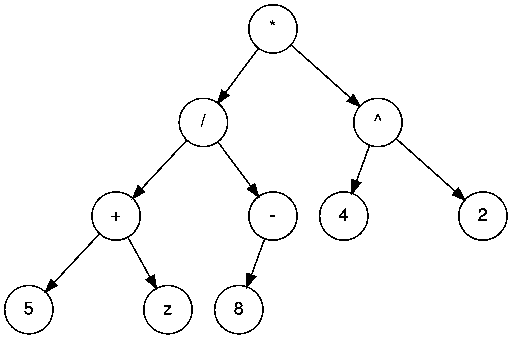
\includegraphics[height=4cm]{2022-1-C2/Exp-tree-ex-12-svg.pdf}
%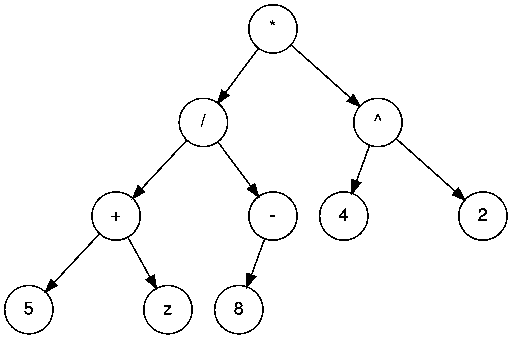
\includegraphics[width=11cm]{2022-1-C2/Exp-tree-ex-12-svg.pdf}

\msk

Ela é a ``expression tree'' correspondente à

expressão $((5+z)/-8)·4^2$.

\msk

a) Descubra qual subárvore dessa figura

corresponde à subexpressão $4^2$.

\msk

a) Cada bolinha dessa figura corresponde a uma

subexpressão da expressão $((5+z)/-8)·4^2$.

Descubra como e diga qual é a expressão

correspondente a cada bolinha.

}\anothercol{
}}



\newpage


%  _____                   _      _         ____  
% | ____|_  _____ _ __ ___(_) ___(_) ___   | ___| 
% |  _| \ \/ / _ \ '__/ __| |/ __| |/ _ \  |___ \ 
% | |___ >  <  __/ | | (__| | (__| | (_) |  ___) |
% |_____/_/\_\___|_|  \___|_|\___|_|\___/  |____/ 
%                                                 
% «exercicio-5»  (to ".exercicio-5")
% (c2m221introp 8 "exercicio-5")
% (c2m221introa   "exercicio-5")


\def\E#1{{\ang{\mathsf{expr_#1}}}}
\def\SA{\bsm{a := b+3 \\ b:=a+4 \\ f(x):=g(x)+5 \\ g(x):=6·x}}
\def\SA{\bsm{a := b+3 \\ b:=a+4 \\ f(x):=g(x)+5 \\ g(x):=6·x}}
\sa{SA}{\bmat{a := b+3 \\ b:=a+4}}
\def\SCa{\bsm{f(x) := \sen x \\ f'(x) := \cos x \\ g(x) := 42x \\ g'(x) := 42}}
\def\Sa{[\mathsf{S1}]}
\def\Sb{[\mathsf{S2}]}
\def\RC{\left( \ddx f(g(x)) = f'(g(x))g'(x) \right)}
\def\RCa{\left( \ddx \sen(42x) = \cos(42x)·42 \right)}
\def\Rc{[\mathsf{RC}]}

\sa{s1}{[\mathsf{S1}]}
\sa{S1}{\bmat{a := b+3 \\ b:=a+4}}


\sa{Rc}{[\mathsf{RC}]}
\sa{RC}{\left( \ddx f(g(x)) = f'(g(x))g'(x) \right)}

\def\r#1{\mathsf{R#1}}

\def\porr#1{\text{(por $\r#1$)}}


\scalebox{0.7}{\def\colwidth{9cm}\firstcol{

$$\D
  \left(
  \frac{a·b+a}{b+2}
  \right) \ga{SA} =
  \left(
  \frac{(b+3)·(a+4)+(b+3)}{(a+4)+2}
  \right)
$$

$$\ga{s1}=\ga{S1}$$

$$\begin{array}{crcl}
  \r1: & (\E1+\E2)\ga{s1} &=& \E1\ga{s1} + \E2\ga{s1} \\
  \r2: & (\E1·\E2)\ga{s1} &=& \E1\ga{s1} · \E2\ga{s1} \\
  \r3: & \D \left(\frac{\E1}{\E2}\right)\ga{s1}
         &=& \D \left( \frac{\E1\ga{s1}}{\E2\ga{s1}} \right) \\
  \r4: & 2 \ga{s1} &=& 2 \\
  \r5: & a \ga{s1} &=& b+3 \\
  \r6: & b \ga{s1} &=& a+4 \\
  \end{array}
$$

$$\begin{array}{rcll}
  (a·b+a)\ga{s1} &=& (a·b)\ga{s1} + a\ga{s1}        & \porr1 \\
                 &=& (a\ga{s1}·b\ga{s1}) + a\ga{s1} & \porr2 \\
                 &=& ((b+3)·b\ga{s1}) + (b+3)       & \porr5 \\
                 &=& ((b+3)·(a+4)) + (b+3)          & \porr6 \\
  \end{array}
$$

}\anothercol{
}}


\newpage

{\bf Exercício 5.}

Calcule
%
$$\D
  \left(
  \frac{a·b+a}{b+2}
  \right) \ga{s1}
$$

bem passo a passo, usando as regras $\r1$ a $\r6$

da página anterior. Arrume o seu cálculo

exatamente no formato descrito aqui,

% (c2m212introp 7 "linguagem")
% (c2m212introa   "linguagem")

\msk

{\footnotesize

% (c2m212introp 7 "linguagem")
% (c2m212introa   "linguagem")
%    http://angg.twu.net/LATEX/2021-2-C2-intro.pdf#page=7
\url{http://angg.twu.net/LATEX/2021-2-C2-intro.pdf#page=7}

}

\msk

em que todos os `$=$'s estão alinhados e a gente

usa uma coluna extra à direita pra dizer a

justificativa de cada `$=$'.



\newpage


%  _____                   _      _          __   
% | ____|_  _____ _ __ ___(_) ___(_) ___    / /_  
% |  _| \ \/ / _ \ '__/ __| |/ __| |/ _ \  | '_ \ 
% | |___ >  <  __/ | | (__| | (__| | (_) | | (_) |
% |_____/_/\_\___|_|  \___|_|\___|_|\___/   \___/ 
%                                                 
% «exercicio-6»  (to ".exercicio-6")
% (c2m221introp 9 "exercicio-6")
% (c2m221introa   "exercicio-6")

\def\Expr{\ang{\mathsf{expr}}}
\def\Just{\ang{\mathsf{justificativa}}}

{\bf Exercício 6.}


\scalebox{0.6}{\def\colwidth{9cm}\firstcol{

No exercício 5 vocês devem ter obtido algo desta forma aqui:

$$\begin{array}{rcll}
    \Expr &=& \Expr & \Just \\
          &=& \Expr & \Just \\
          &=& \Expr & \Just \\
          &=& \Expr & \Just \\
  \end{array}
$$




% «exercicio-6-fig»  (to ".exercicio-6-fig")

Represente cada uma dessas expressões em forma de árvore. A operação
$\Sone$ deve virar uma operação unária, como o `$-$' do `$-8$' na
árvore do Exercício 4. Por exemplo, a representação em árvore de
$(a \Sone + b) \Sone$ vai ser:
%
%
$$%
 \begin{picture}(5.4,5.4)(-1.2,-1.2)%
   \Line(0,0)(3,3) %
   \Line(2,2)(3,1) %
   \putnode(0,0){a} %
   \putnode(1,1){\Sone} %
   \putnode(2,2){+} %
   \putnode(3,3){\Sone} %
   \putnode(3,1){b} %
 \end{picture}%
$$%

}\anothercol{

  O objetivo deste exercício é fazer vocês entenderem este slogan:

  \begin{quote}
    As regras $\r1 \ldots \r6$ empurram os `$\Sone$'s na direção das
    folhas da árvore.
  \end{quote}

}}


\newpage

% «exercicio-7»  (to ".exercicio-7")
% (c2m221introp 10 "exercicio-7")
% (c2m221introa    "exercicio-7")

{\bf Exercício 7.}

\scalebox{0.6}{\def\colwidth{9cm}\firstcol{

    No Exercício 5 você conseguiu se livrar de todos os `$\Sone$'s...
    primeiro você empurrou eles pras folhas, depois você aplicou umas
    regras que fizeram os `$\Sone$'s das folhas sumirem.

    Usando só as regras $\r1\ldots\r6$ a gente não consegue fazer algo
    parecido com a árvore do exercício 4... se a gente tentar
    ``calcular'' isso aqui
    %
    $$(((5+z)/-8)·4^2)\Sone$$

    a gente empaca em vários lugares.

    Repare que o termo ``calcular'' aqui é um abuso de linguagem.
    ``Calcular'' o resultado de $(((5+z)/-8)·4^2)\Sone$ quer dizer
    aplicar as regras $\r1\ldots\r6$ quantas vezes a gente puder, até
    a gente a gente se livrar de todos os `$\Sone$'s. Se a gente
    aplicar as regras $\r1\ldots\r6$ todas as vezes que dá e mesmo
    assim sobre alguns `$\Sone$'s é {\sl como se} faltassem regras pra
    gente ir até o final...

}\anothercol{

  Pra definir a operação $\Stwo$ nós vamos começar tratando as regras
  $\r1\ldots\r4$ da operação $\Sone$ como se elas fossem óbvias ---
  porque elas só ``empurram os `$\Sone$'s na direção das folhas'' ---
  e portanto elas {\sl podem ser deixadas implícitas}.

  A operação $\Stwo$ vai ter só estas duas regras ``explícitas'' aqui,
  %
  $$\begin{array}{crcl}
      \r7: & 8      \Stwo &=& 42 \\
      \r8: & (-\E1) \Stwo &=& 200·(\E1\Stwo) \\
    \end{array}
  $$

  e além disso ela vai ter infinitas regras ``implícitas'' que só
  ``empurram os `$\Stwo$'s na direção das folhas''.

  \bsk

  Tente enteder esta definição informal, e mostre como calcular isto
  % 
  $$(((5+z)/-8)·4^2)\Stwo$$

  bem passo a passo usando as regras do $\Stwo$ --- tanto as duas
  regras explícitas quanto as regras implícitas. Mostre a série de
  passos usando tanto a notação ``algébrica'' acima quanto a notação
  em árvore da figura do exercício 6.




}}




\newpage

% «exercicio-8-intro»  (to ".exercicio-8-intro")
% (c2m221introp 11 "exercicio-8-intro")
% (c2m221introa    "exercicio-8-intro")

{\bf Exercício 8: introdução}


\scalebox{0.8}{\def\colwidth{7cm}\firstcol{

    Lembre que nós estamos lidando com dois tipos de operações de
    substuição: o `$[:=]$' e as operações definidas por regras
    explícitas e implícitas. No exercício 8 nós vamos tentar descobrir
    qual é o modo {\sl certo} de traduzir este `$[:=]$' aqui
    %
    $$\scalebox{0.8}{$
      \begin{array}{l}
        \D \ga{RC} \ga{RCsen(42t) subst} \\
        = \D \ga{RCsen(42t)} \\
      \end{array}
      $}
    $$

    pra uma operação de substituição do segundo tipo... só que antes
    de encontrar a tradução certa nós vamos testar várias traduções
    erradas.

}\anothercol{

    Lembre que se alguém te perguntar qual é o resultado deste
    programa aqui
    %
    $$\text{\tt print("2+2=5")}$$
    %
    a resposta certa é 
    %
    $$\text{\tt 2+2=5}$$
    %
    e não ``esse programa tá errado''...

\msk

As figuras das próximas páginas mostram como a tradução certa deve
funcionar.


}}

\newpage

%L test6_def_nts()
%L Pict2e.bounds = PictBounds.new(v(0,0), v(13,4), 0.5)
%L p = PictList {
%L     nsa(nts_0, "00"),
%L     nsa(nts_1, "01"),
%L     nsa(nts_2, "02"),
%L     nsa(nts_3, "03"),
%L     nsa(nts_4, "04"),
%L   }
%L output(p:tostringp())
\pu


\def\nodesize{0.9}
% \unitlength=35pt

$\ga{00}$
\newpage
$\ga{01}$
\newpage
$\ga{02}$
\newpage
$\ga{03}$
\newpage
$\ga{04}$


\newpage

% «exercicio-8»  (to ".exercicio-8")
% (c2m221introp 17 "exercicio-8")
% (c2m221introa    "exercicio-8")

\def\Sn#1{[\mathsf{S#1}]}
\def\Rn#1{ \mathsf{R#1} }


{\bf Exercício 8.}


\scalebox{0.75}{\def\colwidth{7.5cm}\firstcol{

Lembre que:
%
$$\D \ga{Rc} = \ga{RC}$$

a) Digamos que $\Sn1$ só tem esta regra explícita:
%
$$\begin{array}{lrcl}
  \Rn1: & f(\E1)\Sn1 &=& \sen(\E1) \\
  \end{array}
$$

calcule $\ga{Rc}\Sn1$.

\msk

b) Digamos que $\Sn2$ só tem estas regras explícitas:
%
$$\begin{array}{lrcl}
  \Rn2: & x\Sn2 &=& t \\
  \Rn3: & g'(\E1)\Sn2 &=& \E1 \\
  \end{array}
$$

calcule $\ga{Rc}\Sn2$.

}\anothercol{


c) Digamos que $\Sn3$ só tem estas regras explícitas:
%
$$\begin{array}{lrcl}
  \Rn4: & x\Sn3      &=& t \\
  \Rn5: & f(\E1)\Sn3 &=& \sen(\E1\Sn3) \\
  \Rn6: & f'(\E1)\Sn3 &=& \cos(\E1) \\
  \end{array}
$$

calcule $\ga{Rc}\Sn3$.

}}

% (find-pdf-page "~/2022.1-C2/C2-quadros-tarde.pdf" 4)
% (find-pdf-page "~/2022.1-C2/C2-quadros-manha.pdf")



\newpage

% «exercicio-9»  (to ".exercicio-9")
% (c2m221introp 18 "exercicio-9")
% (c2m221introa    "exercicio-9")

{\bf Exercício 9}

\scalebox{0.65}{\def\colwidth{8.5cm}\firstcol{

    Na página da introdução ao exercício 8 a gente tinha essa figura
    aqui:
    %
    $$\scalebox{0.8}{$
      \begin{array}{l}
        \D \ga{RC} \ga{RCsen(42t) subst} \\
        = \D \ga{RCsen(42t)} \\
      \end{array}
      $}
    $$

    Neste exercício você vai ter que encontrar uma substituição ``do
    segundo tipo'' que obedeça isto:
    %
    $$\scalebox{0.8}{$
      \begin{array}{l}
        \D \ga{RC} \Sn{99} \\
        = \D \ga{RCsen(42t)} \\
      \end{array}
      $}
    $$

    Encontre esta $\Sn{99}$ \ColorRed{por chutar e testar}, no
    seguinte sentido: pra cada um dos seus chutes dê a definição dele
    --- por exemplo, ``Seja $\Sn{20}$ a operação que só tem estas
    regras explícitas: $\ldots$'' --- e depois teste este seu chute,
    ou seja, calcule o resultado de $\ga{Rc}\Sn{20}$.

}\anothercol{

  Se o seu teste não der o resultado que você queria, que é este aqui,
  %
  $$\D \ga{RCsen(42t)}$$

  \ColorRed{não apague} e \ColorRed{não jogue fora} o que você fez. A
  ``resposta'' do exercício 9 deve ser uma série de chutes e testes
  que terminam com uma substituição que dá o resultado ``certo''.

}}



% (find-books "__analysis/__analysis.el" "miranda")
% (find-dmirandacalcpage 87 "3.5 A Regra da Cadeia")




% \newpage
% 
% $$\ga{Rc} = \ga{RC}$$
% 
% $$\RC \SCa = \RCa$$
% 
% $$\D
%   \left(\ddx f(g(x))
%   \frac{a·b+a}{b+2}
%   \right) \SA =
%   \left(
%   \frac{(b+3)·(a+4)+(b+3)}{(a+4)+2}
%   \right)
% $$
% 
% 
% $$\begin{array}{rcl}
%   (a·b+a)\Sa &=& (a·b)\Sa + b\Sa \\
%              &=& (a\Sa·b\Sa) + b\Sa \\
%              &=& (b+3)·(a+4) + (a+4) \\
%   \end{array}
% $$



%\printbibliography

\GenericWarning{Success:}{Success!!!}  % Used by `M-x cv'

\end{document}

%  ____  _             _         
% |  _ \(_)_   ___   _(_)_______ 
% | | | | \ \ / / | | | |_  / _ \
% | |_| | |\ V /| |_| | |/ /  __/
% |____// | \_/  \__,_|_/___\___|
%     |__/                       
%
% «djvuize»  (to ".djvuize")
% (find-LATEXgrep "grep --color -nH --null -e djvuize 2020-1*.tex")

 (eepitch-shell)
 (eepitch-kill)
 (eepitch-shell)
# (find-fline "~/2022.1-C2/")
# (find-fline "~/LATEX/2022-1-C2/")
# (find-fline "~/bin/djvuize")

cd /tmp/
for i in *.jpg; do echo f $(basename $i .jpg); done

f () { rm -v $1.pdf;  textcleaner -f 50 -o  5 $1.jpg $1.png; djvuize $1.pdf; xpdf $1.pdf }
f () { rm -v $1.pdf;  textcleaner -f 50 -o 10 $1.jpg $1.png; djvuize $1.pdf; xpdf $1.pdf }
f () { rm -v $1.pdf;  textcleaner -f 50 -o 20 $1.jpg $1.png; djvuize $1.pdf; xpdf $1.pdf }

f () { rm -fv $1.png $1.pdf; djvuize $1.pdf }
f () { rm -fv $1.png $1.pdf; djvuize WHITEBOARDOPTS="-m 1.0 -f 15" $1.pdf; xpdf $1.pdf }
f () { rm -fv $1.png $1.pdf; djvuize WHITEBOARDOPTS="-m 1.0 -f 30" $1.pdf; xpdf $1.pdf }
f () { rm -fv $1.png $1.pdf; djvuize WHITEBOARDOPTS="-m 1.0 -f 45" $1.pdf; xpdf $1.pdf }
f () { rm -fv $1.png $1.pdf; djvuize WHITEBOARDOPTS="-m 0.5" $1.pdf; xpdf $1.pdf }
f () { rm -fv $1.png $1.pdf; djvuize WHITEBOARDOPTS="-m 0.25" $1.pdf; xpdf $1.pdf }
f () { cp -fv $1.png $1.pdf       ~/2022.1-C2/
       cp -fv        $1.pdf ~/LATEX/2022-1-C2/
       cat <<%%%
% (find-latexscan-links "C2" "$1")
%%%
}

f 20201213_area_em_funcao_de_theta
f 20201213_area_em_funcao_de_x
f 20201213_area_fatias_pizza



%  __  __       _        
% |  \/  | __ _| | _____ 
% | |\/| |/ _` | |/ / _ \
% | |  | | (_| |   <  __/
% |_|  |_|\__,_|_|\_\___|
%                        
% <make>

 (eepitch-shell)
 (eepitch-kill)
 (eepitch-shell)
# (find-LATEXfile "2019planar-has-1.mk")
make -f 2019.mk STEM=2022-1-C2-intro veryclean
make -f 2019.mk STEM=2022-1-C2-intro pdf

% Local Variables:
% coding: utf-8-unix
% ee-tla: "c2i"
% ee-tla: "c2m221intro"
% End:
